\documentclass[a4paper,11pt]{article}

\usepackage[T1]{fontenc}

\usepackage[utf8]{inputenc}

\usepackage[italian]{babel}

\usepackage{graphicx}

\usepackage{indentfirst}

\usepackage{amsmath,amssymb}

\usepackage{enumitem} 

\newcommand{\virgolette}[1]{``#1''}

\usepackage[margin=1in]{geometry} %Smaller margins

\usepackage{lmodern} %Vector PDF

\usepackage{siunitx}

\usepackage{xcolor}

\usepackage{colortbl}

\usepackage{multirow}

\usepackage{rotating}

\usepackage{booktabs}

\usepackage{longtable}

\usepackage{graphicx}
\graphicspath{ {../../Immagini/} }

\usepackage{wrapfig}

\usepackage{siunitx} % Per unità di misura in generale e la corretta rappresentazione dei numeri.

\usepackage{gensymb} % Per il simbolo di gradi

\usepackage{float}

\begin{document}
	
	\section{Analisi e presentazione dei dati}
	Veniamo ora all'analisi dei dati raccolti. Questa operazione si è svolta in quattro fasi:
	
	\begin{enumerate}
		\item Estrazione di c per ogni misura.
		\item Verifica compatibilità dei dati per ogni set.
		\item Stima di c per ogni set di dati.
		\item Verifica compatibilità dei set e media.
	\end{enumerate}
	
	Inoltre le prime due parti dell'analisi dei dati sono state ripetute tre volte, una per ogni set di dati. 
	\subsection{Premesse generale dell'analisi dei dati}
	Nel corso dell'analisi dati ci sono state alcune linee guida seguite per cercare di ottenere il migliore risultato possibile con il minor numero di dati possibili. Poichè erano disponibili diversi dati con diversi errori (per motivi spiegati poi in seguito) questo fine si è ottenuto in primo luogo attraverso l'operazione di media pesata dei dati. Questa statistica è stata preferita alla semplice media in quanto privilegia misure con errore minore senza tuttavia scartare completamente misure con errori più grandi.
	Inoltre l'errore è stato diviso in due parti: \emph{errore sistematico} ed \emph{errore statistico} o \emph{casuale}. Inoltre, tutte le costanti indicate sotto sono relative alla formula \ref{eqn:c}, che per semplicità di lettura è riportata qui sotto.
	\begin{equation*}
	c = \dfrac{4 f_2 D^2 \left(\omega - \omega_0 \right)}{\left(D + a - f_2\right)\Delta\delta}
	\end{equation*}
	\subsubsection{Errore sistematico}
	Per \emph{errore sistematico} si intende un errore nella misura di osservabili utilizzate per ricavare i dati in tutte le misure. In particolare nel ricavare le misure di c sono state usate ripetutamente le misure di, $ D $, la distanza dello specchio rotante dallo specchio concavo, $ a $, la distanza della lente $ 2 $ dallo specchio rotante e $ f_2 $ la distanza focale dello specchio 2. Un errore di misura su una di queste osservabili avrebbe portato ad un errore sistematicamente ripetuto in tutti i calcoli. L'errore finale causato dalla misura di queste osservabili è stato stimato tramite la propagazione degli errori dalla formula \ref{eqn:c} ottenendo quindi che:
	\begin{equation}\label{eqn:sigmac}
		\sigma_{c_{sist}} = \sqrt{\left(\frac{\partial c}{\partial D}\right)^2\sigma_D^2+
			\left(\frac{\partial c}{\partial a}\right)^2\sigma_a^2+\left(\frac{\partial c}{\partial f_2}\right)^2\sigma_{f_2}^2}
	\end{equation}
	dove, per derivazione:
	\begin{equation}\label{eqn:cderivD}
		\frac{\partial c}{\partial D}=\dfrac{4Df_2(2a+D-2f_2)(\omega-\omega_0)}{(a+D-f_2)^2\Delta\delta}
	\end{equation}
	\begin{equation}\label{eqn:deriva}
		\frac{\partial c}{\partial a} = - \dfrac{4D^2f_2(\omega-\omega_0)}{\left(a+D-f_2\right)^2\Delta\delta}
	\end{equation}
	\begin{equation}\label{eqn:derivf2}
		\frac{\partial c}{\partial f_2}=\frac{4D^2(a+D)(\omega-\omega_0)}{(a+d-f_2)^2\Delta\delta}
	\end{equation}
	È stato quindi necessario avere una buona stima dell'errore di queste osservabili. \\
	
	\subsubsection{Errore casuale}
	Gli errori sopra citati non coprono tutti quelli possibili nell'esperimento. In particolare non sono considerati gli errori su $ \Delta\delta $ ne quelli su $ \omega $ e $ \omega_0 $.	Non essendo questi stimabili in modo rigoroso ed essendo idealmente casuali e quindi distribuiti normalmente, gli errori di questi osservabili sono stati raggruppati nella deviazione standard delle misure.
	
	\subsection{Stima delle distanze}\label{sec:dist}
	
	\begin{wraptable}{r} {0.5 \textwidth}
		\centering
		\vspace{-1cm}
		\caption{Misura di $D$}
		\vspace{0.1 cm}
		\begin{tabular}{lrrr}
			\rowcolor[rgb]{ .741,  .843,  .933} \multicolumn{1}{r}{} & \multicolumn{1}{l}{Misura (\si{\meter})} & \multicolumn{1}{l}{Errore (\si{\meter})} & \multicolumn{1}{l}{Err. rel.} \\
			\rowcolor[rgb]{ .741,  .843,  .933} $ D_1 $    & \cellcolor[rgb]{ .859,  .859,  .859} 6.32 & \cellcolor[rgb]{ .859,  .859,  .859} 0.04 & \cellcolor[rgb]{ .859,  .859,  .859} 0.006 \\
			\rowcolor[rgb]{ .741,  .843,  .933} $ D_2 $    & \cellcolor[rgb]{ .929,  .929,  .929} 0.66 & \cellcolor[rgb]{ .929,  .929,  .929} 0.02 & \cellcolor[rgb]{ .929,  .929,  .929} 0.033 \\
			\rowcolor[rgb]{ .741,  .843,  .933} $ D_3 $    & \cellcolor[rgb]{ .859,  .859,  .859} 6.54 & \cellcolor[rgb]{ .859,  .859,  .859} 0.04 & \cellcolor[rgb]{ .859,  .859,  .859} 0.006 \\ 
			\rowcolor[rgb]{ .741,  .843,  .933} $ D $     & \cellcolor[rgb]{ .929,  .929,  .929} 13.52 & \cellcolor[rgb]{ .929,  .929,  .929} 0.35 & \cellcolor[rgb]{ .929,  .929,  .929} 0.026 \\
		\end{tabular}%
		\label{tab:D}
	\end{wraptable}%
	Il valore di $ D $ è stato, tra le distanze, il più complicato da misurare. Questa osservabile è stata calcolata a partire da altre tre osservabili che ai fini del testo chiameremo $ D_1,\ D_2 $ e $ D_3 $. In particolare $ D_1 $ è la distanza tra lo specchio rotante e il centro del primo specchio $ S_1 $, $ D_2 $ è la distanza tra il centro dello specchio $ S_1 $ e il secondo specchio $ S_2 $ e $ D_3 $ è la distanza tra lo specchio $ S_2 $ e lo specchio concavo. In questo modo si ha che:
	\begin{equation}\label{eqn:D}
	D = D_1 + D_2 + D_3 \quad \sigma_D = \sqrt{\sigma_{D_1}^2 + \sigma_{D_2}^2 + \sigma_{D_3}^2}
	\end{equation}
	
	dove $ D $ e $ D_i, \ i=1,2,3 $ sono come prima e $ \sigma_D $ e $ \sigma_{D_i}, \ i=1,2,3 $ sono gli errori delle relative misure. L'errore di queste distanze derivava da molti fattori, in particolar modo causati dallo strumento di misura. Come descritto nelle sezioni precedenti queste misure sono state effettuate con il metro a nastro, con sensibilità al centimetro. La principale fonte di errore derivava dal fatto che il metro, sospeso in aria, si fletteva sotto al proprio peso modificando il valore letto. Un'altra fonte di errore è stata la non perfetta centratura del metro, dovuta anche al fatto che non era possibile toccare le superfici degli specchi.
	Con queste considerazioni, si sono stimati, in base alla variabilità delle possibili misure sono riportati nella tabella \ref{tab:D}.
	
	\begin{wraptable}{l} {0.5 \textwidth}
		\vspace{-0.5cm}
		\centering
		\caption{Misura di $ a $}
		\vspace{0.1cm}
		\begin{tabular}{lrrr}
			\rowcolor[rgb]{ .741,  .843,  .933}       & \multicolumn{1}{l}{Misura (\si{\meter})} & \multicolumn{1}{l}{Errore (\si{\meter})} & \multicolumn{1}{l}{Err. rel.} \\
			\rowcolor[rgb]{ .741,  .843,  .933} $s_{f_2}$ & \cellcolor[rgb]{ .859,  .859,  .859} 0.252 & \cellcolor[rgb]{ .859,  .859,  .859} 0.001 & \cellcolor[rgb]{ .859,  .859,  .859} 0.004 \\
			\rowcolor[rgb]{ .741,  .843,  .933} $s_{spr}$ & \cellcolor[rgb]{ .929,  .929,  .929} 0.865 & \cellcolor[rgb]{ .929,  .929,  .929} 0.005 & \cellcolor[rgb]{ .929,  .929,  .929} 0.006 \\
			\rowcolor[rgb]{ .741,  .843,  .933} $a$   & \cellcolor[rgb]{ .859,  .859,  .859} 0.478 & \cellcolor[rgb]{ .859,  .859,  .859} 0.005 & \cellcolor[rgb]{ .859,  .859,  .859} 0.011 \\
		\end{tabular}%
		\label{tab:a}%
	\end{wraptable}%
	
	
	In confronto a $ D $, la stima dell'errore di $ a $ è stata più semplice. Come mostrato nelle figure \ref{photo 6} e \ref{photo 7}, sia la lente che lo specchio rotante si trovavano su una guida sulla quale era incollato un metro. Mentre la lente aveva un chiaro riferimento per la posizione (una piccola tacchetta bianca) lo specchio rotante no. Per questa ragione per lo specchio è stata aumentata l'incertezza di misura da $ \SI{1}{\milli\meter} $ a $ \SI{5}{\milli\meter} $. Quindi $ a $ è stata calcolata attraverso la seguente relazione:
	\begin{equation}\label{eqn:a}
	a = s_{spr} - s_{f_2} \quad \sigma_a = \sqrt{ \sigma_{s_{spr}}^2+\sigma_{s_{f_2}}^2}
	\end{equation}
	dove $ s_{spr} $ è la posizione dello specchio rotante, $ s_{f_2} $ è la posizione della lente 2 e le altre costanti sono i relativi errori. I valori misurati e i rispettivi errori sono presenti in tabella \ref{tab:a}.
	
	Non c'è stata una vera e propria misura di $ f_2 $ poiché questo valore era dato dal costruttore. Come errore è stato considerato un millesimo del valore. Quindi:
	\[ 
	f_2 = \SI{0.242}{\meter} \quad \sigma_{f_2}=\SI{0.242 e-4}{\meter}
	\]
	\subsection{Estrazione della velocità per ogni misura}
	Come anticipato nel corso dell'esperimento sono stati effettuati tre set di misura: uno facendo ruotare lo specchio in senso orario (set \emph{clockwise}), uno in senso antiorario (set \emph{counterclockwise}) e uno facendolo partire in senso antiorario e finendo in senso orario (set \emph{counterclock-clock}). Per ogni misura si sono quindi campionati i valori di $ \nu,\, \nu_0$ (che attraverso la relazione $ \omega=2\pi\nu $ si sono convertiti rispettivamente in $ \omega $ e $ \omega_0 $ ), $\delta_1, $ e $ \delta_2 $. Il valore di $ \Delta\delta $ è stato calcolato come differenza di $ \delta_1 $ e $ \delta_2 $. Il valore di $ c $ per ogni misura è stato calcolato tramite la formula \ref{eqn:c} e i valori ricavati nella sezione \ref{sec:dist}. Sono di seguito riportate le misure campionate, con i relativi valori di $ c $ e gli errori sistematici.\footnote{Per la tabella \ref{tab:couterclockclockdata}, è stata usata una convenzione per cui frequenze di rotazioni antiorarie sono state considerate negative.}
	
	\begin{table}[htbp]
		\centering
		\caption{Set \emph{clockwise}}
		\vspace{0.1cm}
		\begin{tabular}{rllllllr}
			\rowcolor[rgb]{ .741,  .843,  .933} \multicolumn{1}{l}{Indice} & $\nu_0$ (\si{\hertz}) & $\nu$ (\si{\hertz}) & $\delta_1$ (\si{\milli\meter}) & $\delta_2$ (\si{\milli\meter}) & $c$ (\si{\meter\per\second}) & $\sigma_{sist}$ (\si{\meter\per\second}) & \multicolumn{1}{l}{Err. Rel.} \\
			\rowcolor[rgb]{ .741,  .843,  .933} 1     & \cellcolor[rgb]{ .859,  .859,  .859} \num{82} & \cellcolor[rgb]{ .859,  .859,  .859} \num{934} & \cellcolor[rgb]{ .859,  .859,  .859} \num{09.94} & \cellcolor[rgb]{ .859,  .859,  .859} \num{10.17} & \cellcolor[rgb]{ .859,  .859,  .859} \num{326.16E+06} & \cellcolor[rgb]{ .859,  .859,  .859} \num{8.50E+06} & \cellcolor[rgb]{ .859,  .859,  .859} 0.039 \\
			\rowcolor[rgb]{ .741,  .843,  .933} 2     & \cellcolor[rgb]{ .929,  .929,  .929} \num{110} & \cellcolor[rgb]{ .929,  .929,  .929} \num{917} & \cellcolor[rgb]{ .929,  .929,  .929} \num{09.94} & \cellcolor[rgb]{ .929,  .929,  .929} \num{10.18} & \cellcolor[rgb]{ .929,  .929,  .929} \num{311.98E+06} & \cellcolor[rgb]{ .929,  .929,  .929} \num{8.13E+06} & \cellcolor[rgb]{ .929,  .929,  .929} 0.040 \\
			\rowcolor[rgb]{ .741,  .843,  .933} 3     & \cellcolor[rgb]{ .859,  .859,  .859} \num{108} & \cellcolor[rgb]{ .859,  .859,  .859} \num{959} & \cellcolor[rgb]{ .859,  .859,  .859} \num{09.95} & \cellcolor[rgb]{ .859,  .859,  .859} \num{10.18} & \cellcolor[rgb]{ .859,  .859,  .859} \num{283.19E+06} & \cellcolor[rgb]{ .859,  .859,  .859} \num{7.38E+06} & \cellcolor[rgb]{ .859,  .859,  .859} 0.042 \\
			\rowcolor[rgb]{ .741,  .843,  .933} 4     & \cellcolor[rgb]{ .929,  .929,  .929} \num{100} & \cellcolor[rgb]{ .929,  .929,  .929} \num{929} & \cellcolor[rgb]{ .929,  .929,  .929} \num{09.95} & \cellcolor[rgb]{ .929,  .929,  .929} \num{10.18} & \cellcolor[rgb]{ .929,  .929,  .929} \num{311.62E+06} & \cellcolor[rgb]{ .929,  .929,  .929} \num{8.12E+06} & \cellcolor[rgb]{ .929,  .929,  .929} 0.040 \\
			\rowcolor[rgb]{ .741,  .843,  .933} 5     & \cellcolor[rgb]{ .859,  .859,  .859} \num{118} & \cellcolor[rgb]{ .859,  .859,  .859} \num{1002} & \cellcolor[rgb]{ .859,  .859,  .859} \num{09.94} & \cellcolor[rgb]{ .859,  .859,  .859} \num{10.20} & \cellcolor[rgb]{ .859,  .859,  .859} \num{303.56E+06} & \cellcolor[rgb]{ .859,  .859,  .859} \num{7.91E+06} & \cellcolor[rgb]{ .859,  .859,  .859} 0.040 \\
			\rowcolor[rgb]{ .741,  .843,  .933} 6     & \cellcolor[rgb]{ .929,  .929,  .929} \num{115} & \cellcolor[rgb]{ .929,  .929,  .929} \num{1435} & \cellcolor[rgb]{ .929,  .929,  .929} \num{09.94} & \cellcolor[rgb]{ .929,  .929,  .929} \num{10.31} & \cellcolor[rgb]{ .929,  .929,  .929} \num{286.35E+06} & \cellcolor[rgb]{ .929,  .929,  .929} \num{7.46E+06} & \cellcolor[rgb]{ .929,  .929,  .929} 0.042 \\
			\rowcolor[rgb]{ .741,  .843,  .933} 7     & \cellcolor[rgb]{ .859,  .859,  .859} \num{100} & \cellcolor[rgb]{ .859,  .859,  .859} \num{977} & \cellcolor[rgb]{ .859,  .859,  .859} \num{09.94} & \cellcolor[rgb]{ .859,  .859,  .859} \num{10.20} & \cellcolor[rgb]{ .859,  .859,  .859} \num{300.46E+06} & \cellcolor[rgb]{ .859,  .859,  .859} \num{7.83E+06} & \cellcolor[rgb]{ .859,  .859,  .859} 0.041 \\
			\rowcolor[rgb]{ .741,  .843,  .933} 8     & \cellcolor[rgb]{ .929,  .929,  .929} \num{107} & \cellcolor[rgb]{ .929,  .929,  .929} \num{900} & \cellcolor[rgb]{ .929,  .929,  .929} \num{09.94} & \cellcolor[rgb]{ .929,  .929,  .929} \num{10.16} & \cellcolor[rgb]{ .929,  .929,  .929} \num{284.08E+06} & \cellcolor[rgb]{ .929,  .929,  .929} \num{7.40E+06} & \cellcolor[rgb]{ .929,  .929,  .929} 0.042 \\
			\rowcolor[rgb]{ .741,  .843,  .933} 9     & \cellcolor[rgb]{ .859,  .859,  .859} \num{109} & \cellcolor[rgb]{ .859,  .859,  .859} \num{950} & \cellcolor[rgb]{ .859,  .859,  .859} \num{09.94} & \cellcolor[rgb]{ .859,  .859,  .859} \num{10.19} & \cellcolor[rgb]{ .859,  .859,  .859} \num{303.58E+06} & \cellcolor[rgb]{ .859,  .859,  .859} \num{7.91E+06} & \cellcolor[rgb]{ .859,  .859,  .859} 0.040 \\
			\rowcolor[rgb]{ .741,  .843,  .933} 10    & \cellcolor[rgb]{ .929,  .929,  .929} \num{119} & \cellcolor[rgb]{ .929,  .929,  .929} \num{1442} & \cellcolor[rgb]{ .929,  .929,  .929} \num{09.95} & \cellcolor[rgb]{ .929,  .929,  .929} \num{10.33} & \cellcolor[rgb]{ .929,  .929,  .929} \num{283.32E+06} & \cellcolor[rgb]{ .929,  .929,  .929} \num{7.38E+06} & \cellcolor[rgb]{ .929,  .929,  .929} 0.042 \\
			\rowcolor[rgb]{ .741,  .843,  .933} 11    & \cellcolor[rgb]{ .859,  .859,  .859} \num{120} & \cellcolor[rgb]{ .859,  .859,  .859} \num{1440} & \cellcolor[rgb]{ .859,  .859,  .859} \num{09.94} & \cellcolor[rgb]{ .859,  .859,  .859} \num{10.33} & \cellcolor[rgb]{ .859,  .859,  .859} \num{293.22E+06} & \cellcolor[rgb]{ .859,  .859,  .859} \num{7.64E+06} & \cellcolor[rgb]{ .859,  .859,  .859} 0.041 \\
			\rowcolor[rgb]{ .741,  .843,  .933} 12    & \cellcolor[rgb]{ .929,  .929,  .929} \num{102} & \cellcolor[rgb]{ .929,  .929,  .929} \num{1420} & \cellcolor[rgb]{ .929,  .929,  .929} \num{09.94} & \cellcolor[rgb]{ .929,  .929,  .929} \num{10.30} & \cellcolor[rgb]{ .929,  .929,  .929} \num{288.76E+06} & \cellcolor[rgb]{ .929,  .929,  .929} \num{7.53E+06} & \cellcolor[rgb]{ .929,  .929,  .929} 0.042 \\
			\rowcolor[rgb]{ .741,  .843,  .933} 13    & \cellcolor[rgb]{ .859,  .859,  .859} \num{127} & \cellcolor[rgb]{ .859,  .859,  .859} \num{1435} & \cellcolor[rgb]{ .859,  .859,  .859} \num{09.95} & \cellcolor[rgb]{ .859,  .859,  .859} \num{10.31} & \cellcolor[rgb]{ .859,  .859,  .859} \num{308.34E+06} & \cellcolor[rgb]{ .859,  .859,  .859} \num{8.04E+06} & \cellcolor[rgb]{ .859,  .859,  .859} 0.040 \\
			\rowcolor[rgb]{ .741,  .843,  .933} 14    & \cellcolor[rgb]{ .929,  .929,  .929} \num{114} & \cellcolor[rgb]{ .929,  .929,  .929} \num{1436} & \cellcolor[rgb]{ .929,  .929,  .929} \num{09.94} & \cellcolor[rgb]{ .929,  .929,  .929} \num{10.31} & \cellcolor[rgb]{ .929,  .929,  .929} \num{306.00E+06} & \cellcolor[rgb]{ .929,  .929,  .929} \num{7.98E+06} & \cellcolor[rgb]{ .929,  .929,  .929} 0.040 \\
			\rowcolor[rgb]{ .741,  .843,  .933} 15    & \cellcolor[rgb]{ .859,  .859,  .859} \num{107} & \cellcolor[rgb]{ .859,  .859,  .859} \num{1422} & \cellcolor[rgb]{ .859,  .859,  .859} \num{09.95} & \cellcolor[rgb]{ .859,  .859,  .859} \num{10.32} & \cellcolor[rgb]{ .859,  .859,  .859} \num{300.92E+06} & \cellcolor[rgb]{ .859,  .859,  .859} \num{7.84E+06} & \cellcolor[rgb]{ .859,  .859,  .859} 0.041 \\
			\rowcolor[rgb]{ .741,  .843,  .933} 16    & \cellcolor[rgb]{ .929,  .929,  .929} \num{109} & \cellcolor[rgb]{ .929,  .929,  .929} \num{1443} & \cellcolor[rgb]{ .929,  .929,  .929} \num{09.95} & \cellcolor[rgb]{ .929,  .929,  .929} \num{10.33} & \cellcolor[rgb]{ .929,  .929,  .929} \num{299.32E+06} & \cellcolor[rgb]{ .929,  .929,  .929} \num{7.80E+06} & \cellcolor[rgb]{ .929,  .929,  .929} 0.041 \\
			\rowcolor[rgb]{ .741,  .843,  .933} 17    & \cellcolor[rgb]{ .859,  .859,  .859} \num{144} & \cellcolor[rgb]{ .859,  .859,  .859} \num{1422} & \cellcolor[rgb]{ .859,  .859,  .859} \num{09.96} & \cellcolor[rgb]{ .859,  .859,  .859} \num{10.32} & \cellcolor[rgb]{ .859,  .859,  .859} \num{295.66E+06} & \cellcolor[rgb]{ .859,  .859,  .859} \num{7.71E+06} & \cellcolor[rgb]{ .859,  .859,  .859} 0.041 \\
			\rowcolor[rgb]{ .741,  .843,  .933} 18    & \cellcolor[rgb]{ .929,  .929,  .929} \num{128} & \cellcolor[rgb]{ .929,  .929,  .929} \num{1433} & \cellcolor[rgb]{ .929,  .929,  .929} \num{09.94} & \cellcolor[rgb]{ .929,  .929,  .929} \num{10.32} & \cellcolor[rgb]{ .929,  .929,  .929} \num{298.98E+06} & \cellcolor[rgb]{ .929,  .929,  .929} \num{7.79E+06} & \cellcolor[rgb]{ .929,  .929,  .929} 0.041 \\
			\rowcolor[rgb]{ .741,  .843,  .933} 19    & \cellcolor[rgb]{ .859,  .859,  .859} \num{119} & \cellcolor[rgb]{ .859,  .859,  .859} \num{1440} & \cellcolor[rgb]{ .859,  .859,  .859} \num{09.95} & \cellcolor[rgb]{ .859,  .859,  .859} \num{10.33} & \cellcolor[rgb]{ .859,  .859,  .859} \num{289.23E+06} & \cellcolor[rgb]{ .859,  .859,  .859} \num{7.54E+06} & \cellcolor[rgb]{ .859,  .859,  .859} 0.042 \\
		\end{tabular}%
		\label{tab:clockdata}%
	\end{table}%
		
	\begin{table}[htbp]
		\centering
		\caption{Set \emph{counterclockwise}}
		\vspace{0.1cm}
		\begin{tabular}{rllllllr}
			\rowcolor[rgb]{ .741,  .843,  .933} \multicolumn{1}{l}{Indice} & $\nu_0$ (\si{\hertz}) & $\nu$ (\si{\hertz}) & $\delta_1$ (\si{\milli\meter}) & $\delta_2$ (\si{\milli\meter}) & $c$ (\si{\meter\per\second}) & $\sigma_{sist}$ (\si{\meter\per\second}) & \multicolumn{1}{l}{Err. Rel.} \\
			\rowcolor[rgb]{ .741,  .843,  .933} 1     & \cellcolor[rgb]{ .859,  .859,  .859} \num{118} & \cellcolor[rgb]{ .859,  .859,  .859} \num{920} & \cellcolor[rgb]{ .859,  .859,  .859} \num{09.87} & \cellcolor[rgb]{ .859,  .859,  .859} \num{09.66} & \cellcolor[rgb]{ .859,  .859,  .859} \num{321.64E+06} & \cellcolor[rgb]{ .859,  .859,  .859} \num{8.38E+06} & \cellcolor[rgb]{ .859,  .859,  .859} 0.049 \\
			\rowcolor[rgb]{ .741,  .843,  .933} 2     & \cellcolor[rgb]{ .929,  .929,  .929} \num{114} & \cellcolor[rgb]{ .929,  .929,  .929} \num{908} & \cellcolor[rgb]{ .929,  .929,  .929} \num{09.88} & \cellcolor[rgb]{ .929,  .929,  .929} \num{09.65} & \cellcolor[rgb]{ .929,  .929,  .929} \num{290.74E+06} & \cellcolor[rgb]{ .929,  .929,  .929} \num{7.58E+06} & \cellcolor[rgb]{ .929,  .929,  .929} 0.053 \\
			\rowcolor[rgb]{ .741,  .843,  .933} 3     & \cellcolor[rgb]{ .859,  .859,  .859} \num{127} & \cellcolor[rgb]{ .859,  .859,  .859} \num{915} & \cellcolor[rgb]{ .859,  .859,  .859} \num{09.86} & \cellcolor[rgb]{ .859,  .859,  .859} \num{09.65} & \cellcolor[rgb]{ .859,  .859,  .859} \num{316.03E+06} & \cellcolor[rgb]{ .859,  .859,  .859} \num{8.24E+06} & \cellcolor[rgb]{ .859,  .859,  .859} 0.050 \\
			\rowcolor[rgb]{ .741,  .843,  .933} 4     & \cellcolor[rgb]{ .929,  .929,  .929} \num{115} & \cellcolor[rgb]{ .929,  .929,  .929} \num{908} & \cellcolor[rgb]{ .929,  .929,  .929} \num{09.88} & \cellcolor[rgb]{ .929,  .929,  .929} \num{09.65} & \cellcolor[rgb]{ .929,  .929,  .929} \num{290.38E+06} & \cellcolor[rgb]{ .929,  .929,  .929} \num{7.57E+06} & \cellcolor[rgb]{ .929,  .929,  .929} 0.053 \\
			\rowcolor[rgb]{ .741,  .843,  .933} 5     & \cellcolor[rgb]{ .859,  .859,  .859} \num{97} & \cellcolor[rgb]{ .859,  .859,  .859} \num{963} & \cellcolor[rgb]{ .859,  .859,  .859} \num{09.87} & \cellcolor[rgb]{ .859,  .859,  .859} \num{09.62} & \cellcolor[rgb]{ .859,  .859,  .859} \num{291.74E+06} & \cellcolor[rgb]{ .859,  .859,  .859} \num{7.60E+06} & \cellcolor[rgb]{ .859,  .859,  .859} 0.053 \\
			\rowcolor[rgb]{ .741,  .843,  .933} 6     & \cellcolor[rgb]{ .929,  .929,  .929} \num{79} & \cellcolor[rgb]{ .929,  .929,  .929} \num{1400} & \cellcolor[rgb]{ .929,  .929,  .929} \num{09.88} & \cellcolor[rgb]{ .929,  .929,  .929} \num{09.53} & \cellcolor[rgb]{ .929,  .929,  .929} \num{317.87E+06} & \cellcolor[rgb]{ .929,  .929,  .929} \num{8.29E+06} & \cellcolor[rgb]{ .929,  .929,  .929} 0.050 \\
			\rowcolor[rgb]{ .741,  .843,  .933} 7     & \cellcolor[rgb]{ .859,  .859,  .859} \num{115} & \cellcolor[rgb]{ .859,  .859,  .859} \num{1395} & \cellcolor[rgb]{ .859,  .859,  .859} \num{09.88} & \cellcolor[rgb]{ .859,  .859,  .859} \num{09.54} & \cellcolor[rgb]{ .859,  .859,  .859} \num{317.07E+06} & \cellcolor[rgb]{ .859,  .859,  .859} \num{8.26E+06} & \cellcolor[rgb]{ .859,  .859,  .859} 0.050 \\
			\rowcolor[rgb]{ .741,  .843,  .933} 8     & \cellcolor[rgb]{ .929,  .929,  .929} \num{113} & \cellcolor[rgb]{ .929,  .929,  .929} \num{1385} & \cellcolor[rgb]{ .929,  .929,  .929} \num{09.89} & \cellcolor[rgb]{ .929,  .929,  .929} \num{09.54} & \cellcolor[rgb]{ .929,  .929,  .929} \num{306.08E+06} & \cellcolor[rgb]{ .929,  .929,  .929} \num{7.98E+06} & \cellcolor[rgb]{ .929,  .929,  .929} 0.051 \\
			\rowcolor[rgb]{ .741,  .843,  .933} 9     & \cellcolor[rgb]{ .859,  .859,  .859} \num{79} & \cellcolor[rgb]{ .859,  .859,  .859} \num{1396} & \cellcolor[rgb]{ .859,  .859,  .859} \num{09.88} & \cellcolor[rgb]{ .859,  .859,  .859} \num{09.54} & \cellcolor[rgb]{ .859,  .859,  .859} \num{326.23E+06} & \cellcolor[rgb]{ .859,  .859,  .859} \num{8.50E+06} & \cellcolor[rgb]{ .859,  .859,  .859} 0.049 \\
			\rowcolor[rgb]{ .741,  .843,  .933} 10    & \cellcolor[rgb]{ .929,  .929,  .929} \num{93} & \cellcolor[rgb]{ .929,  .929,  .929} \num{1385} & \cellcolor[rgb]{ .929,  .929,  .929} \num{09.89} & \cellcolor[rgb]{ .929,  .929,  .929} \num{09.54} & \cellcolor[rgb]{ .929,  .929,  .929} \num{310.89E+06} & \cellcolor[rgb]{ .929,  .929,  .929} \num{8.10E+06} & \cellcolor[rgb]{ .929,  .929,  .929} 0.051 \\
		\end{tabular}%
		\label{tab:counterclockdata}%
	\end{table}%
	
	\begin{table}[htbp]
		\centering
		\caption{Set \emph{counterclock-clockwise}}
		\vspace{0.1cm}		
		\begin{tabular}{rllllllr}
			\rowcolor[rgb]{ .741,  .843,  .933} \multicolumn{1}{l}{Indice} & $\nu_0$ (\si{\hertz}) & $\nu$ (\si{\hertz}) & $\delta_1$ (\si{\milli\meter}) & $\delta_2$ (\si{\milli\meter}) & $c$ (\si{\meter\per\second}) & $\sigma_{sist}$ (\si{\meter\per\second}) & \multicolumn{1}{l}{Err. Rel.} \\
			\rowcolor[rgb]{ .741,  .843,  .933} 1     & \cellcolor[rgb]{ .859,  .859,  .859} \num{-1384} & \cellcolor[rgb]{ .859,  .859,  .859} \num{1384} & \cellcolor[rgb]{ .859,  .859,  .859} \num{10.32} & \cellcolor[rgb]{ .859,  .859,  .859} \num{09.53} & \cellcolor[rgb]{ .859,  .859,  .859} \num{296.97E+06} & \cellcolor[rgb]{ .859,  .859,  .859} \num{7.74E+06} & \cellcolor[rgb]{ .859,  .859,  .859} 0.029 \\
			\rowcolor[rgb]{ .741,  .843,  .933} 2     & \cellcolor[rgb]{ .929,  .929,  .929} \num{-1388} & \cellcolor[rgb]{ .929,  .929,  .929} \num{1382} & \cellcolor[rgb]{ .929,  .929,  .929} \num{10.31} & \cellcolor[rgb]{ .929,  .929,  .929} \num{09.54} & \cellcolor[rgb]{ .929,  .929,  .929} \num{302.97E+06} & \cellcolor[rgb]{ .929,  .929,  .929} \num{7.90E+06} & \cellcolor[rgb]{ .929,  .929,  .929} 0.029 \\
			\rowcolor[rgb]{ .741,  .843,  .933} 3     & \cellcolor[rgb]{ .859,  .859,  .859} \num{-1395} & \cellcolor[rgb]{ .859,  .859,  .859} \num{1373} & \cellcolor[rgb]{ .859,  .859,  .859} \num{10.32} & \cellcolor[rgb]{ .859,  .859,  .859} \num{09.53} & \cellcolor[rgb]{ .859,  .859,  .859} \num{293.24E+06} & \cellcolor[rgb]{ .859,  .859,  .859} \num{7.64E+06} & \cellcolor[rgb]{ .859,  .859,  .859} 0.029 \\
			\rowcolor[rgb]{ .741,  .843,  .933} 4     & \cellcolor[rgb]{ .929,  .929,  .929} \num{-1410} & \cellcolor[rgb]{ .929,  .929,  .929} \num{1395} & \cellcolor[rgb]{ .929,  .929,  .929} \num{10.33} & \cellcolor[rgb]{ .929,  .929,  .929} \num{09.53} & \cellcolor[rgb]{ .929,  .929,  .929} \num{293.46E+06} & \cellcolor[rgb]{ .929,  .929,  .929} \num{7.65E+06} & \cellcolor[rgb]{ .929,  .929,  .929} 0.029 \\
			\rowcolor[rgb]{ .741,  .843,  .933} 5     & \cellcolor[rgb]{ .859,  .859,  .859} \num{-1405} & \cellcolor[rgb]{ .859,  .859,  .859} \num{1397} & \cellcolor[rgb]{ .859,  .859,  .859} \num{10.32} & \cellcolor[rgb]{ .859,  .859,  .859} \num{09.53} & \cellcolor[rgb]{ .859,  .859,  .859} \num{298.72E+06} & \cellcolor[rgb]{ .859,  .859,  .859} \num{7.79E+06} & \cellcolor[rgb]{ .859,  .859,  .859} 0.029 \\
			\rowcolor[rgb]{ .741,  .843,  .933} 6     & \cellcolor[rgb]{ .929,  .929,  .929} \num{-1416} & \cellcolor[rgb]{ .929,  .929,  .929} \num{1396} & \cellcolor[rgb]{ .929,  .929,  .929} \num{10.32} & \cellcolor[rgb]{ .929,  .929,  .929} \num{09.52} & \cellcolor[rgb]{ .929,  .929,  .929} \num{296.03E+06} & \cellcolor[rgb]{ .929,  .929,  .929} \num{7.72E+06} & \cellcolor[rgb]{ .929,  .929,  .929} 0.029 \\
			\rowcolor[rgb]{ .741,  .843,  .933} 7     & \cellcolor[rgb]{ .859,  .859,  .859} \num{-1420} & \cellcolor[rgb]{ .859,  .859,  .859} \num{1394} & \cellcolor[rgb]{ .859,  .859,  .859} \num{10.32} & \cellcolor[rgb]{ .859,  .859,  .859} \num{09.53} & \cellcolor[rgb]{ .859,  .859,  .859} \num{301.91E+06} & \cellcolor[rgb]{ .859,  .859,  .859} \num{7.87E+06} & \cellcolor[rgb]{ .859,  .859,  .859} 0.029 \\
			\rowcolor[rgb]{ .741,  .843,  .933} 8     & \cellcolor[rgb]{ .929,  .929,  .929} \num{-1428} & \cellcolor[rgb]{ .929,  .929,  .929} \num{1399} & \cellcolor[rgb]{ .929,  .929,  .929} \num{10.34} & \cellcolor[rgb]{ .929,  .929,  .929} \num{09.54} & \cellcolor[rgb]{ .929,  .929,  .929} \num{299.49E+06} & \cellcolor[rgb]{ .929,  .929,  .929} \num{7.81E+06} & \cellcolor[rgb]{ .929,  .929,  .929} 0.029 \\
			\rowcolor[rgb]{ .741,  .843,  .933} 9     & \cellcolor[rgb]{ .859,  .859,  .859} \num{-1416} & \cellcolor[rgb]{ .859,  .859,  .859} \num{1398} & \cellcolor[rgb]{ .859,  .859,  .859} \num{10.35} & \cellcolor[rgb]{ .859,  .859,  .859} \num{09.55} & \cellcolor[rgb]{ .859,  .859,  .859} \num{296.25E+06} & \cellcolor[rgb]{ .859,  .859,  .859} \num{7.72E+06} & \cellcolor[rgb]{ .859,  .859,  .859} 0.029 \\
			\rowcolor[rgb]{ .741,  .843,  .933} 10    & \cellcolor[rgb]{ .929,  .929,  .929} \num{-1420} & \cellcolor[rgb]{ .929,  .929,  .929} \num{1395} & \cellcolor[rgb]{ .929,  .929,  .929} \num{10.32} & \cellcolor[rgb]{ .929,  .929,  .929} \num{09.53} & \cellcolor[rgb]{ .929,  .929,  .929} \num{302.01E+06} & \cellcolor[rgb]{ .929,  .929,  .929} \num{7.87E+06} & \cellcolor[rgb]{ .929,  .929,  .929} 0.029 \\
		\end{tabular}%
		\label{tab:couterclockclockdata}%
	\end{table}%
	\newpage
	\subsection{Verifica bontà dei dati acquisiti}
	A questo punto, prima di estrarre da ogni set la misura della velocità della luce è stato necessario verificare la compatibilità dei dati sotto alle ipotesi di errori effettuate e verificarne l'indipendenza. Tutti i controlli di indipendenza sono stati effettuati con un \emph{confidence level} del $ 95\% $ rispetto alla variabile standardizzata $ z $ di Gauss. 
	
	\subsubsection{Verifica compatibilità} \label{subsubsec:vercomp}
	Per applicare correttamente l'operazione di media pesata è necessario verificare che i valori che si mediano siano compatibili, ossia derivino dalla stessa distribuzione. Come era facile aspettarsi, il controllo di compatibilità tra le misure dei set effettuato con solo l'errore sistematico (quello tabulato nelle tabelle \ref{tab:clockdata}, \ref{tab:counterclockdata} e \ref{tab:couterclockclockdata}). Per controllare la compatibilità era necessario aggiungere all'errore anche la componente casuale. Si è scelto, come prima stima dell'errore casuale, la deviazione standard delle misure di $ c $ del set. I valori delle deviazioni standard sono riportati in tabella \ref{tab:setdevstd}.
	

	\begin{table}[htbp]
		\centering
		\caption{Deviazioni standard dei set}
		\vspace{0.1cm}
		\begin{tabular}{llll}
			\rowcolor[rgb]{ .741,  .843,  .933}       & \emph{Clockwise} & \emph{Counterclockwise} & \emph{Counterclock-clockwise} \\
			\rowcolor[rgb]{ .741,  .843,  .933} Dev. Std. (\si{\meter}) & \cellcolor[rgb]{ .859,  .859,  .859} \num{9.40E6} & \cellcolor[rgb]{ .859,  .859,  .859} \num{13.50E6} & \cellcolor[rgb]{ .859,  .859,  .859} \num{3.50E6} \\
		\end{tabular}%
		\label{tab:setdevstd}%
	\end{table}%
	
	Questa statistica è stata preferita rispetto alla deviazione standard della media in quanto ogni valore era preso da un campione solo di dati e non era frutto di alcuna medi: con questa operazione non si voleva verificare che i valori siano statisticamente uguali, ma che derivino da una stessa distribuzione. A causa della quantità di dati confrontati, e delle dimensioni occupate da una tabella che riporti tali valori, queste non saranno ricopiate. Con i dati sopra il lettore interessato può verificare che tutte le misure sono compatibili in questo modo. Sono però riportati nelle figure \ref{fig:clockwiseplot}, \ref{fig:counterclockwiseplot} e \ref{fig:clock-anticlockplot} seguenti i valori misurati con gli errori ottenuti e, come confronto, la misura reale della velocità della luce.
	
	\begin{figure}
		\centering
		\caption{\emph{Clockwise} data set}
		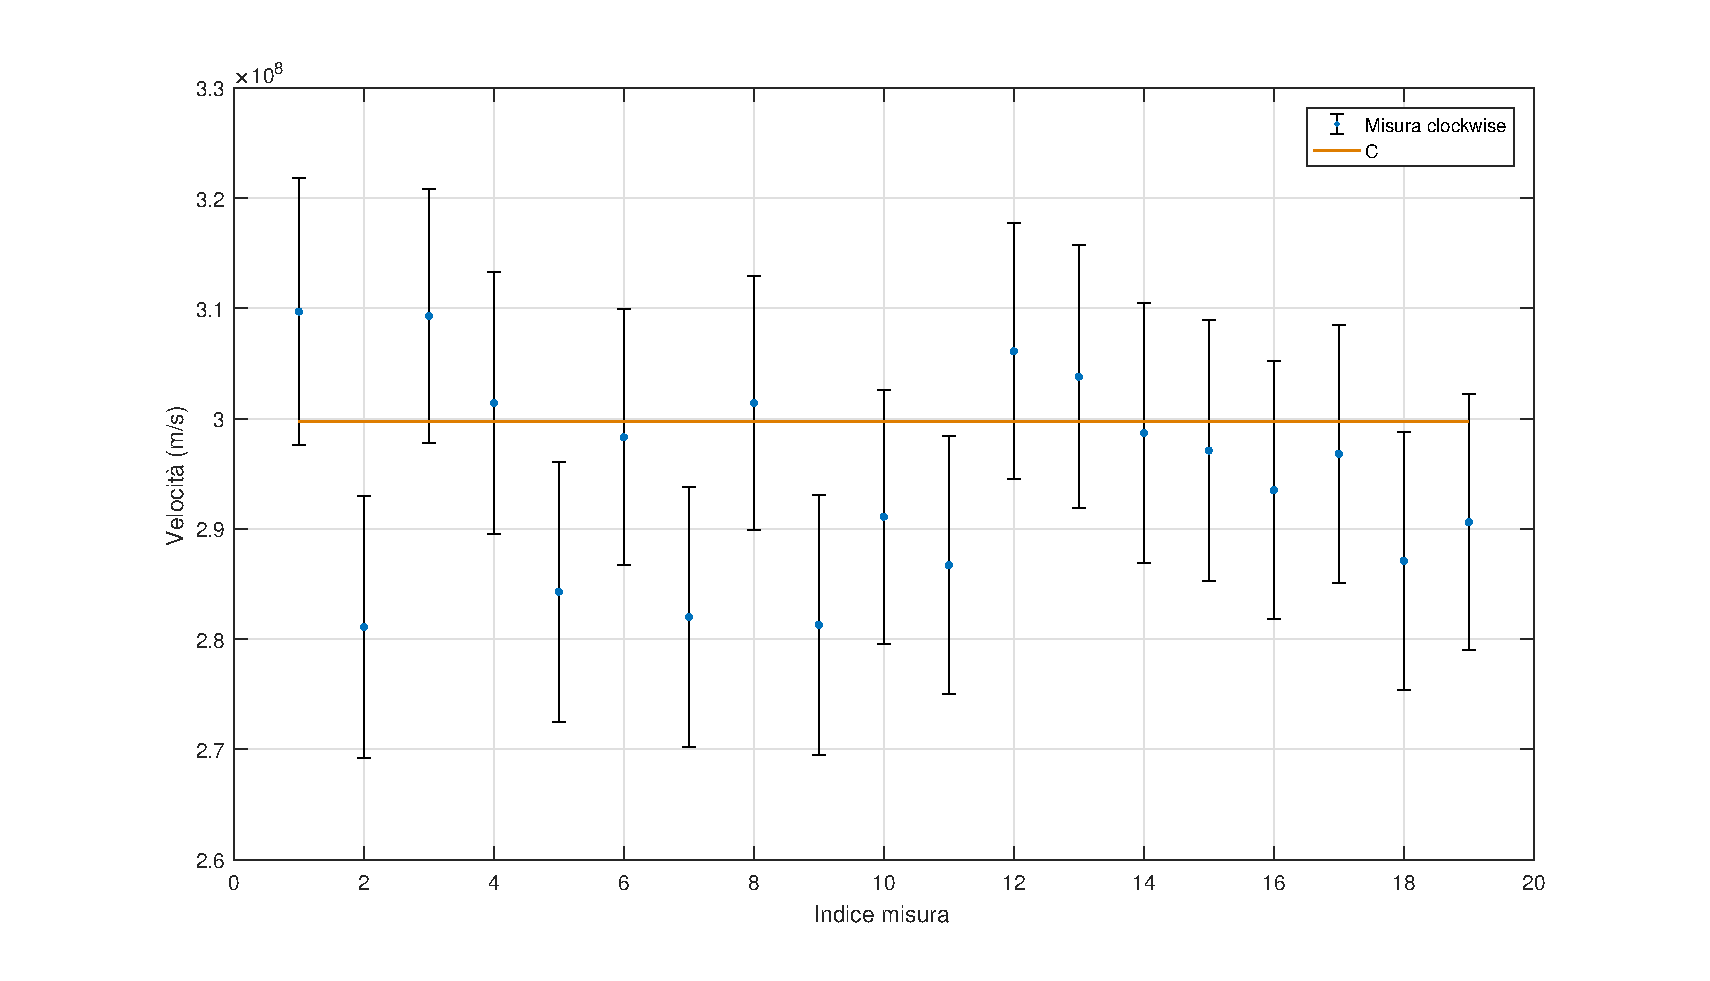
\includegraphics[width=.98\textwidth]{Clockwiseplot}
		\label{fig:clockwiseplot}
	\end{figure}
	

	\begin{figure}
		\centering
		\caption{\emph{Counterclockwise} data set}
		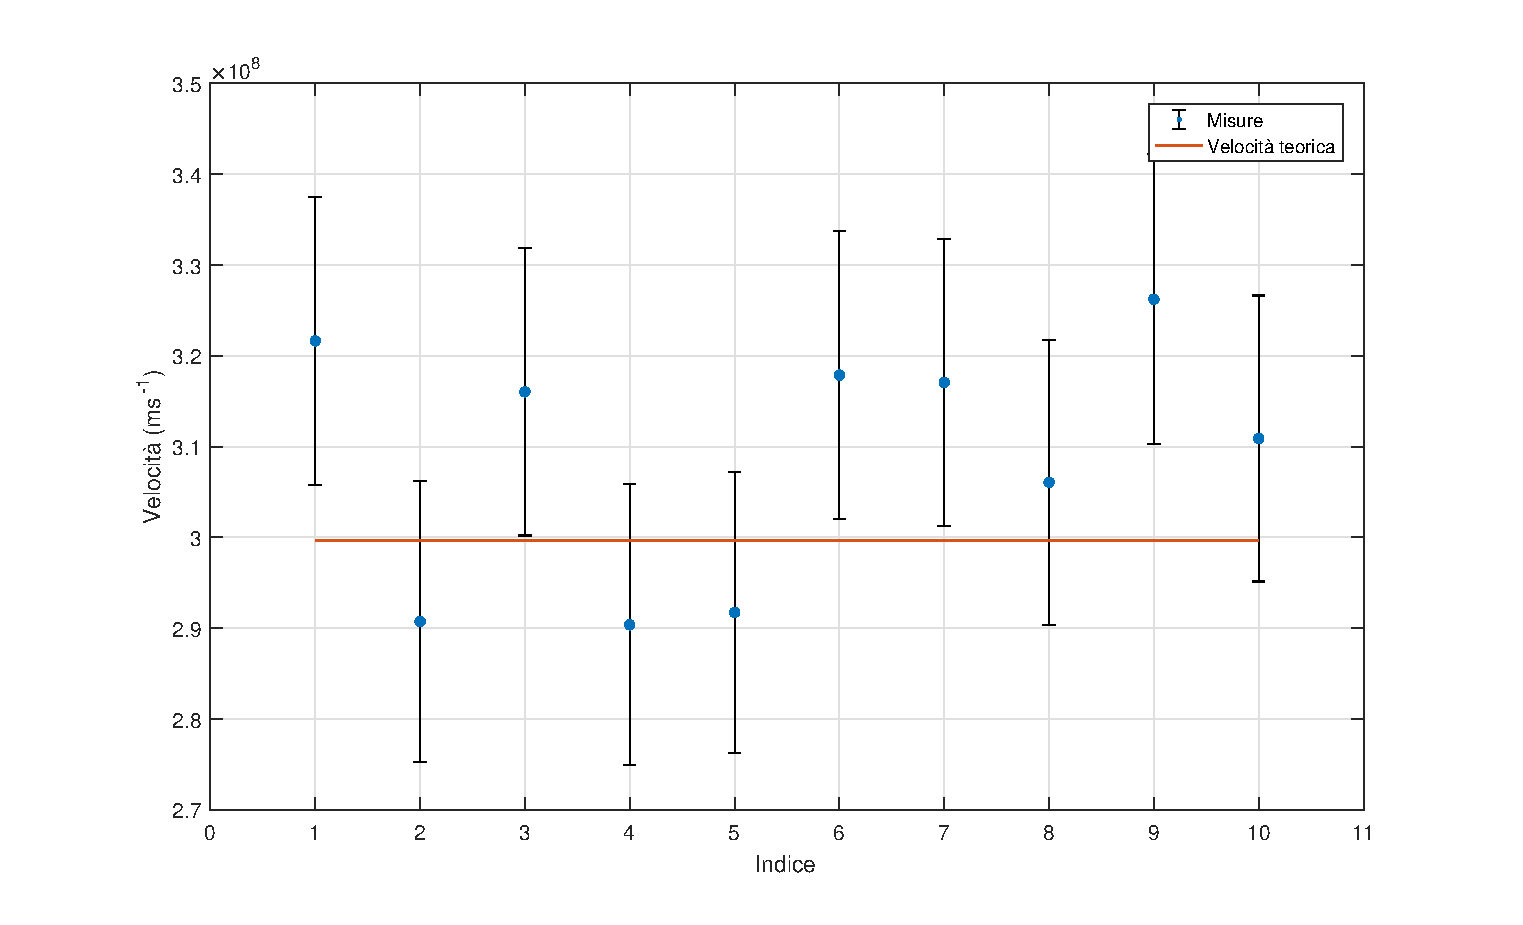
\includegraphics[width=.98\textwidth]{Counterclockwiseplot}
		\label{fig:counterclockwiseplot}
	\end{figure}
	
	\begin{figure}
		\centering
		\caption{\emph{Counterclock-clockwise} data set}
		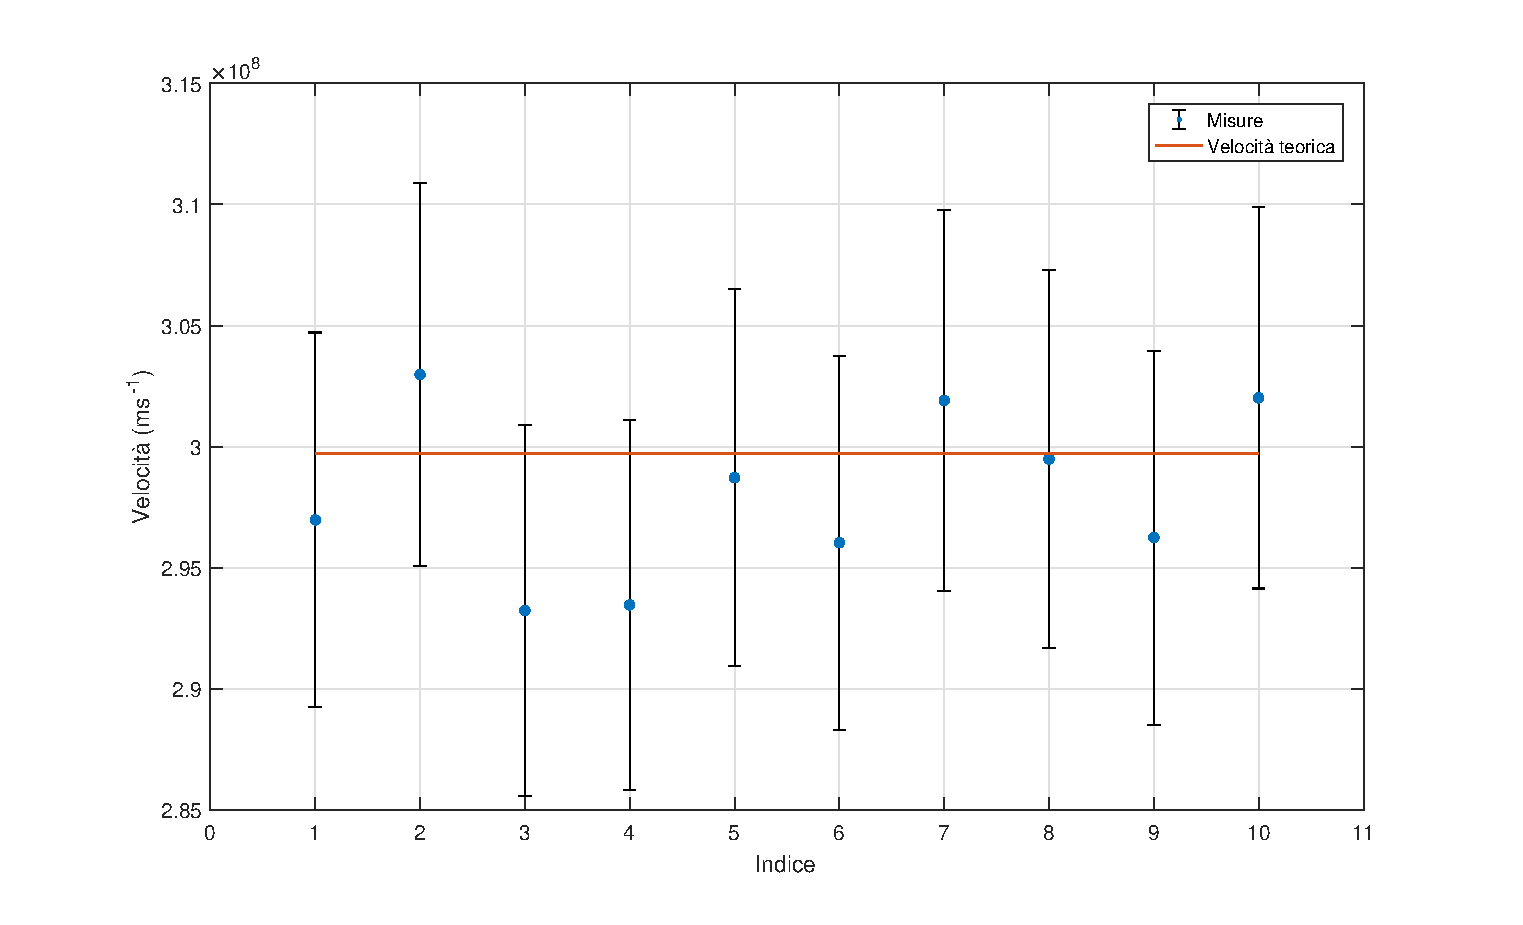
\includegraphics[width=.98\textwidth]{Clock-anticlockplot}
		\label{fig:clock-anticlockplot}
	\end{figure}
	\subsubsection{Verifica indipendenza}
	Per la verifica dell'indipendenza dei dati si è usato il valore teorico della velocità della luce. In particolare un set di dati indipendenti avrebbe prodotto una distribuzione normale di valori della velocità della luce misurati centrati nel valore teorico e con deviazione standard uguale all'errore totale stimato. Per provare questa ipotesi si è usato il test del $ \chi^2 $. Come errore è stato usato lo stesso errore descritto nella sezione \ref{subsubsec:vercomp}. In tutti e tre i casi il test ha verificato l'ipotesi di indipendenza. A seguito di queste due operazioni è dunque lecito eseguire l'operazione di media pesata.
	\subsection{Stima della velocità della luce per ogni set}
	Come anticipato per la stima della velocità della luce è stata eseguita una media pesata 
	
	
	\end{document}